% Created 2016-08-17 Wed 14:38
\documentclass[tikz]{standalone}

\usepackage[utf8]{inputenc}
\usepackage[T1]{fontenc}
\usepackage{helvet}
\usepackage{../../templates/msc}

\renewcommand{\familydefault}{\sfdefault}

\tikzset{
every picture/.style={
line width=1pt
}}

\usepackage{tikz}
\author{Holger Karl}
\date{\today}
\title{}

\usetikzlibrary{arrows.meta,
                calc, chains,
                quotes,
                positioning,
                shapes.geometric}

\begin{document}

  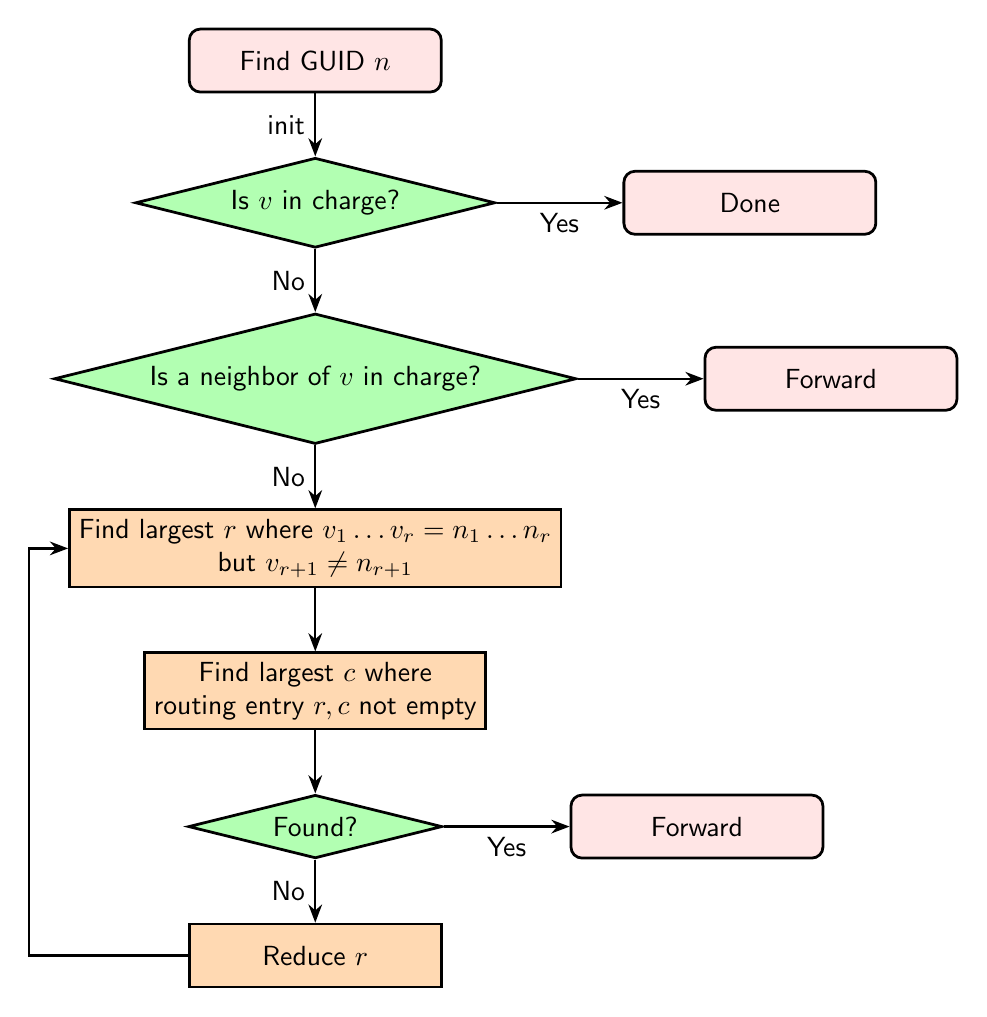
\begin{tikzpicture}[
    node distance = 8mm and 16mm,
      start chain = A going below,
      base/.style = {draw, minimum width=32mm, minimum height=8mm,
                     align=center, on chain=A},
 startstop/.style = {base, rectangle, rounded corners, fill=red!10},
   process/.style = {base, rectangle, fill=orange!30},
        io/.style = {base, trapezium, 
                     trapezium left angle=70, trapezium right angle=110,
                     fill=blue!30},
  decision/.style = {base, diamond, fill=green!30, aspect=4},
  every edge quotes/.style = {auto=right}]
                    ]
\node [startstop]       {Find GUID $n$};            % <-- A-1
\node [decision]        { Is $v$ in charge?}; 
\node [startstop, right=of A-2]         {Done};       
\node [decision, below=of A-2]        { Is a neighbor of $v$ in charge?}; 
\node [startstop, right=of A-4]         {Forward};       
\node [process, below=of A-4]         {Find largest $r$ where $v_1\ldots v_r = n_1\ldots n_r$ \\ but $v_{r+1} \not = n_{r+1}$ }; 
% 
\node [process]                                  {Find largest $c$ where \\ routing entry $r, c$ not empty}; 
\node [decision] {Found?};
\node [startstop, right=of A-8]  {Forward};
\node [process, below=of A-8]  {Reduce $r$};
%%
\draw [arrows=-Stealth,thick] 
    (A-1) edge["init"]          (A-2)
    (A-2) edge["Yes"]    (A-3) 
    (A-2) edge["No"]    (A-4) 
    (A-4) edge["Yes"]    (A-5) 
    (A-4) edge["No"]    (A-6) 
    (A-6) edge    (A-7) 
    (A-7) edge    (A-8) 
    (A-8) edge["Yes"]    (A-9) 
    (A-8) edge["No"]    (A-10) 
    (A-10.west) -|   ([xshift=-0.5cm]A-6.west) --     (A-6.west);
  \end{tikzpicture}



\end{document}